\section{Transistor Amplifiers}\label{sec:Transistor_Amps}
Now, we are going to apply \emph{both} AC and DC signals to a \nameref{def:Transistor}, and watch the outputs.
There is some important terminology to be aware of here:
\begin{description}
\item[DC] Uses all uppercase letters, such as $\DCVoltage{\Base}$ or $\DCCurrent{\Drain}$.
\item[AC] Uses all lowercase letters, such as $\ACVoltage{\Gate\Source}$ or $\ACCurrent{\Drain}$.
\item[Mixed] Uses lowercase letters, with capital subscripts, such as $\SignalVoltage{GS}$.
  These are typically defined as $\SignalVoltage{GS} = \ACVoltage{GS} + \DCVoltage{GS}$.
\end{description}

To solve a transistor amplifier problem, there are a few steps:
\begin{enumerate}[noitemsep]
\item Find the DC bias point of the \nameref{def:Transistor}.
  This involves performing DC analysis of the transistor, like was done in \Cref{sec:MOSFETs} and \Cref{sec:BJTs}.
  Zero \emph{all} AC sources and treat all capacitors as open circuits.
  \begin{enumerate}[noitemsep]
  \item When solving, assume the \nameref{def:Transistor} is in the useful region for amplification.
  \end{enumerate}
\item Find the transconductance gain, $\TransconductanceGain$ of the circuit (\Cref{eq:MOSFET-Transconductance_Gain,eq:BJT-Transconductance_Gain}).
\item Find the AC operation of the \nameref{def:Transistor}.
  This involves performing AC analysis of the transistor.
  Zero \emph{all} DC sources, and treat all capacitors are short circuits.
\item Make use of a small-signal equivalent circuit.
\end{enumerate}

\subsection{Biasing}\label{subsec:Biasing}
Biasing of a \nameref{def:Transistor} is required so that it is operating in its active region (\nameref{subsubsec:MOSFET_Saturation_Region} for \nameref{def:MOSFET}s, and \nameref{subsubsec:BJT_Active_Region} for \nameref{def:BJT}s).

If we view the $\ACVoltage{\Gate\Source}$-$\ACVoltage{\Drain\Source}$ voltage transfer characteristics of a \nameref{def:MOSFET} (\Cref{fig:MOSFET-Bias_Graph}) or the $\ACVoltage{\Base\Emitter}$-$\ACVoltage{\Collector\Emitter}$ voltage transfer characteristic of a \nameref{def:BJT} (\Cref{fig:BJT-Bias_Graph}), we can see why this is necessary.

\begin{figure}[h!tbp]
  \centering
  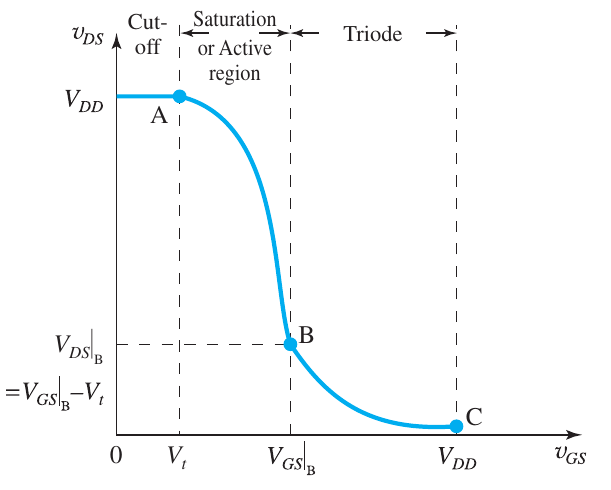
\includegraphics[scale=0.85]{./MOSFET-Bias_Graph.png}
  \caption{\nameref*{def:MOSFET} Voltage Transfer Characteristic}
  \label{fig:MOSFET-Bias_Graph}
\end{figure}

\begin{figure}[h!tbp]
  \centering
  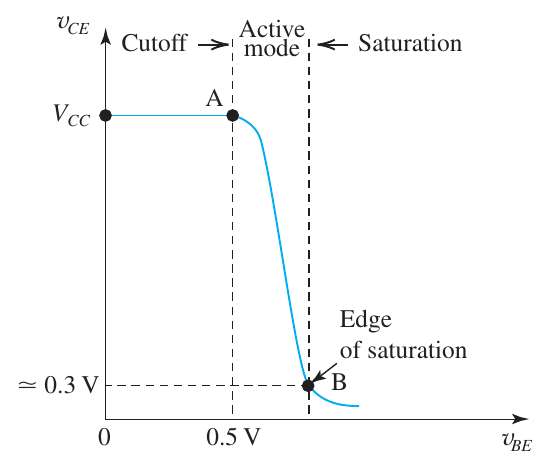
\includegraphics[scale=0.85]{./BJT-Bias_Graph.png}
  \caption{\nameref*{def:BJT} Voltage Transfer Characteristic}
  \label{fig:BJT-Bias_Graph}
\end{figure}

For a \nameref{def:Transistor} to properly amplify a given input signal, it must have a non-constant voltage-transfer characteristic, otherwise the amplifier does nothing.
Thus, the \nameref{def:Transistor} \textbf{must} be in its active region for anything to happen.
If the transistor were to enter either its cutoff or saturation modes, then the input signal would become distorted at the output.
See \Cref{fig:MOSFET-Bias_Transfer_Characteristic} for an example/visualization of how this works.

\begin{figure}[h!tbp]
  \centering
  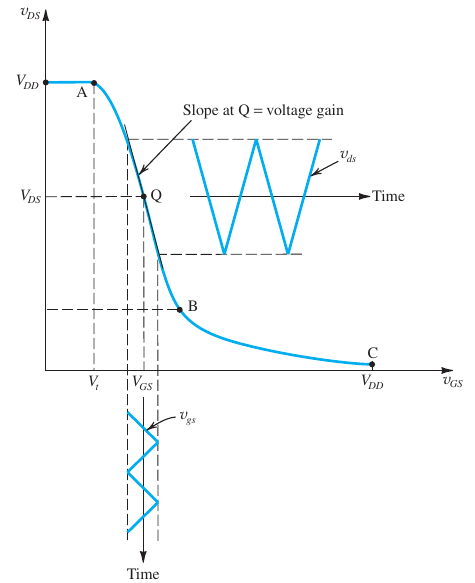
\includegraphics[scale=0.65]{./MOSFET-Bias_Transfer_Characteristic.png}
  \caption[\nameref*{def:MOSFET} Transfer Graph]{\nameref*{def:MOSFET} Voltage Transfer Characteristic Superimposed with Input Signal}
  \label{fig:MOSFET-Bias_Transfer_Characteristic}
\end{figure}

This means that \nameref{def:Transistor}s \textbf{must} be biased with a DC voltage to operate in the appropriate region, but they must not be too close to any edge.
If they are too close to an edge, the input AC signal will make the bias point leave the active region of the \nameref{def:Transistor}, causing the output signal to be distorted.

\begin{definition}[Quiescent Point]\label{def:Quiescent_Point}
  The \emph{quiescent point} is a given biasing point in the transfer function of a voltage transfer characteristic.
  If you calculate a bias point, and it is \emph{not} the maximum bias point for that signal, then it is called a quiescent point.
  The quiescent point is denoted with $\QuiescentPoint$.
\end{definition}

\nameref{def:Quiescent_Point}s are denoted with $\QuiescentPoint$, and the maximum bias point is $\MaxBiasPoint$.

\subsection{MOSFET Amplifiers}\label{subsec:MOSFET_Amps}
The \nameref{def:Transconductance_Gain} is defined in \Cref{def:Transconductance_Gain}, and its defining equations are shown in \Cref{eq:MOSFET-Transconductance_Gain}.

\begin{definition}[Transconductance Gain]\label{def:Transconductance_Gain}
  The \emph{(open-circuit) transconductance gain}, $\TransconductanceGain$ is the transconductance that the \nameref{def:Transistor} experiences when operating in its DC mode.
  It is defined to two different equations depending on the \nameref{def:Transistor} used.
  \begin{description}[noitemsep]
  \item[\nameref{def:MOSFET}] \Cref{eq:MOSFET-Transconductance_Gain}
  \item[\nameref{def:BJT}] \Cref{eq:BJT-Transconductance_Gain}
  \end{description}
\end{definition}

\Crefrange{eq:MOSFET-Transconductance_Gain-Overdrive_Voltage}{eq:MOSFET-Transconductance_Gain-Drain_Current_Overdrive_Voltage} provide all the possible equations one can use to find the \nameref{def:Transconductance_Gain} of a \nameref{def:MOSFET}.

\begin{subequations}\label{eq:MOSFET-Transconductance_Gain}
  \begin{equation}\label{eq:MOSFET-Transconductance_Gain-Overdrive_Voltage}
    \TransconductanceGain = \ElectronMobility \OxideCapacitivity \frac{\Width}{\Length} \OverdriveVoltage
  \end{equation}
  \begin{equation}\label{eq:MOSFET-Transconductance_Gain-Drain_Current}
    \TransconductanceGain = \sqrt{2 \ElectronMobility \OxideCapacitivity \frac{\Width}{\Length} \DCCurrent{\Drain}}
  \end{equation}
  \begin{equation}\label{eq:MOSFET-Transconductance_Gain-Drain_Current_Overdrive_Voltage}
    \TransconductanceGain = \frac{2 \DCCurrent{\Drain}}{\OverdriveVoltage}
  \end{equation}
\end{subequations}

The small-signal open circuit voltage gain of a \nameref{def:MOSFET} is given in \Cref{eq:MOSFET-Small_Signal_Voltage_Gain}, and the maximum value is found in \Cref{eq:MOSFET-Small_Signal_Voltage_Gain-Max}.
\begin{equation}\label{eq:MOSFET-Small_Signal_Voltage_Gain}
  \Amp{\Voltage} = -\frac{\DCVoltage{DD} - \DCVoltage{DS}}{\frac{\OverdriveVoltage}{2}}
\end{equation}

\begin{equation}\label{eq:MOSFET-Small_Signal_Voltage_Gain-Max}
  \Abs{\Amp{\Voltage,Max}} = \frac{\DCVoltage{DD} - \left. \OverdriveVoltage \right\rvert_{\MaxBiasPoint}}{\frac{\left. \OverdriveVoltage \right\rvert_{\MaxBiasPoint}}{2}}
\end{equation}

In addition to \Cref{eq:MOSFET-Small_Signal_Voltage_Gain}, the small-signal amplification of a \nameref{def:MOSFET} is also dependent on several factors of the circuit, as shown in \Cref{eq:MOSFET-Small_Signal_Voltage_Gain-Overdrive_Voltage}.
\begin{equation}\label{eq:MOSFET-Small_Signal_Voltage_Gain-Overdrive_Voltage}
  \Amp{\Voltage} = -k_{\NType} R_{\Drain} \OverdriveVoltage
\end{equation}

The resistance at the output \emph{due to the inefficiencies of the transistor} is defined by \Cref{eq:MOSFET-Transistor_Resistance}.
\begin{equation}\label{eq:MOSFET-Transistor_Resistance}
  \ChannelModResist = \frac{\DCVoltage{A}}{\DCCurrent{\Drain}}
\end{equation}
This resistance goes in \emph{parallel} with the voltage-dependent current source that the \nameref{def:Transistor} can be modeled as, see \Cref{fig:MOSFET-Small_Signal_Model-ro}.

\subsubsection{Small-Signal Models}\label{subsubsec:MOSFET-Small_Signal_Models}
\Cref{fig:MOSFET-Small_Signal_Model} is the simplest model we can use.
In it, we neglect the dependence of $\ACCurrent{\Drain}$ on $\ACVoltage{\Drain\Source}$, \nameref{subsubsec:MOSFET-Early_Effect}.

\begin{figure}[h!tbp]
  \centering
  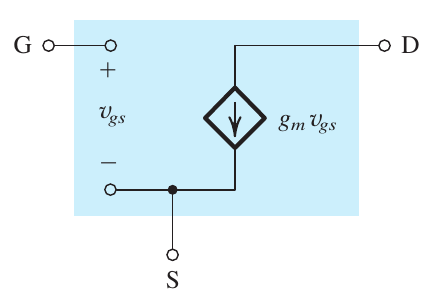
\includegraphics[scale=0.65]{./MOSFET-Small_Signal_Model.png}
  \caption{Small Signal Model of MOSFET \parencite[p.~387]{sedraTextbook7}}
  \label{fig:MOSFET-Small_Signal_Model}
\end{figure}

\Cref{fig:MOSFET-Small_Signal_Model-ro} is a more accurate model of a \nameref{def:MOSFET}.
It includes the resistance due to the \nameref{def:Transistor}'s channel length modulation, \nameref{subsubsec:MOSFET-Early_Effect}.
\Cref{eq:MOSFET-Transistor_Resistance} is the value of $\ChannelModResist$.

\begin{figure}[h!tbp]
  \centering
  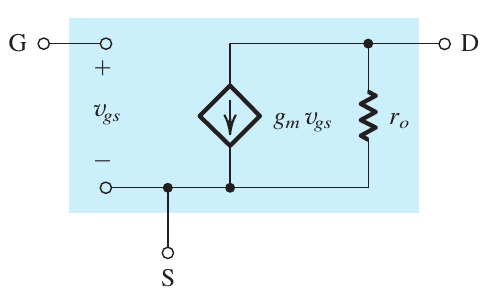
\includegraphics[scale=0.65]{./MOSFET-Small_Signal_Model-ro.png}
  \caption{Small Signal Model of MOSFET, including Channel Modulation Resistance \parencite[p.~387]{sedraTextbook7}}
  \label{fig:MOSFET-Small_Signal_Model-ro}
\end{figure}

An alternative set of models drawn from the first two small-signal models (\Cref{fig:MOSFET-Small_Signal_Model,fig:MOSFET-Small_Signal_Model-ro}) is the T-Model, \Cref{fig:MOSFET-T_Small_Signal_Model,fig:MOSFET-T_Small_Signal_Model-ro}.

\begin{figure}[h!tbp]
  \centering
  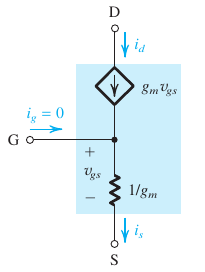
\includegraphics[scale=0.85]{./MOSFET-T_Small_Signal_Model.png}
  \caption{T-Model Equivalent of \nameref*{def:MOSFET} \parencite[p.~394]{sedraTextbook7}}
  \label{fig:MOSFET-T_Small_Signal_Model}
\end{figure}

\begin{figure}[h!tbp]
  \centering
  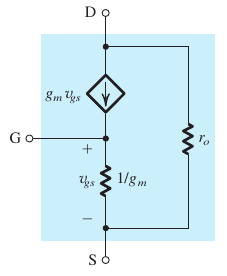
\includegraphics[scale=0.85]{./MOSFET-T_Small_Signal_Model-ro.png}
  \caption{T-Model Equivalent of \nameref*{def:MOSFET}, including Channel Modulation Resistance \parencite[p.~395]{sedraTextbook7}}
  \label{fig:MOSFET-T_Small_Signal_Model-ro}
\end{figure}

\begin{remark*}[Why T-Model?]
  The T-models are preferred when there is a resistor attached to the source of the \nameref{def:MOSFET}.
\end{remark*}

\subsubsection{Configurations}\label{subsubsec:MOSFET_Configurations}
There are three possible configurations for a \nameref{def:MOSFET}, as seen in \Crefrange{fig:MOSFET-Common_Source}{fig:MOSFET-Common_Drain}.

\begin{figure}[h!tbp]
  \centering
  \begin{subfigure}{0.30\linewidth}
    \centering
    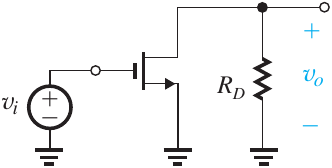
\includegraphics[scale=0.50]{./MOSFET-Common_Source.png}
    \caption{Common Source Configuration\\\parencite[p.~424]{sedraTextbook7}}
    \label{fig:MOSFET-Common_Source}
  \end{subfigure}
  \begin{subfigure}{0.30\linewidth}
    \centering
    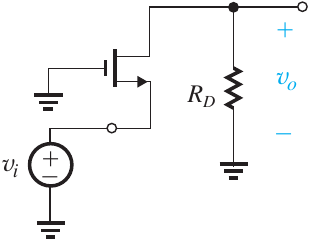
\includegraphics[scale=0.50]{./MOSFET-Common_Gate.png}
    \caption{Common Gate Configuration\\\parencite[p.~424]{sedraTextbook7}}
    \label{fig:MOSFET-Common_Gate}
  \end{subfigure}
  \begin{subfigure}{0.30\linewidth}
    \centering
    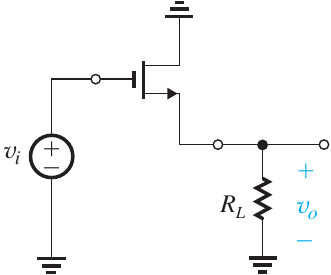
\includegraphics[scale=0.50]{./MOSFET-Common_Drain.png}
    \caption{Common Drain Configuration\\\parencite[p.~424]{sedraTextbook7}}
    \label{fig:MOSFET-Common_Drain}
  \end{subfigure}
  \caption{\nameref*{def:MOSFET} Configurations}
  \label{fig:MOSFET_Configurations}
\end{figure}

\subsection{BJT Amplifiers}\label{subsec:BJT_Amps}
The \nameref{def:Transconductance_Gain} of a \nameref{def:BJT} is given by \Cref{eq:BJT-Transconductance_Gain}.
\begin{equation}\label{eq:BJT-Transconductance_Gain}
  \TransconductanceGain = \frac{\DCCurrent{\Collector}}{\ThermalVoltage}
\end{equation}

Then, the resistance due to the channel modulation resistance is given by \Cref{eq:BJT-Transistor_Resistance}.
\begin{equation}\label{eq:BJT-Transistor_Resistance}
  \ChannelModResist = \frac{\Abs{\DCVoltage{A}}}{\DCCurrent{\Collector}}
\end{equation}

Lastly, the resistances from the \nameref{def:BJT}'s construction is \Cref{eq:BJT-Emitter_Resistance,eq:BJT-Pi_Resistance}.
\begin{equation}\label{eq:BJT-Emitter_Resistance}
  r_{e} = \frac{\ThermalVoltage}{\DCCurrent{\Emitter}} = \alpha \frac{\ThermalVoltage}{\DCCurrent{\Collector}}
\end{equation}

\begin{equation}\label{eq:BJT-Pi_Resistance}
  r_{\pi} = \frac{\ThermalVoltage}{\DCCurrent{\Base}} = \beta \frac{\ThermalVoltage}{\DCCurrent{C}}
\end{equation}

The small-signal voltage gain of a \nameref{def:BJT} is shown in \Cref{eq:BJT-Small_Signal_Voltage_Gain}.
\begin{equation}\label{eq:BJT-Small_Signal_Voltage_Gain}
  \Amp{V} = - \frac{\DCCurrent{\Collector} R_{\Collector}}{\ThermalVoltage}
\end{equation}

\subsubsection{Small-Signal Models}\label{subsubsec:BJT-Small_Signal_Models}
\Crefrange{fig:BJT-Hybrid_Pi_Model-vbe}{fig:BJT-T_Model-ib} are small-signal equivalents for a \nameref{def:BJT}.
This is for an ideal \nameref{def:BJT}, but a realistic one includes the channel modulation resistance, $\ChannelModResist$.
\Crefrange{fig:BJT-Hybrid_Pi_Model-vbe-ro}{fig:BJT-T_Model-ib-ro} are the equivalent circuits with the channel length resistance included.

\begin{figure}[h!tbp]
  \centering
  \begin{subfigure}{0.45\linewidth}
    \centering
    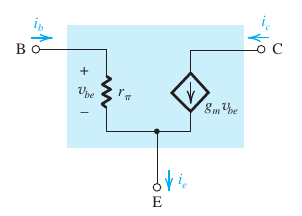
\includegraphics[scale=0.75]{./BJT-Hybrid_Pi-vbe.png}
    \caption{Hybrid-$\pi$ Model Small-Signal Model, using $\ACVoltage{\pi}$\\\parencite[p.~407]{sedraTextbook7}}
    \label{fig:BJT-Hybrid_Pi_Model-vbe}
  \end{subfigure}
  \begin{subfigure}{0.45\linewidth}
    \centering
    \includegraphics[scale=0.75]{./BJT-Hybrid_Pi-beta_ib.png}
    \caption{Hybrid-$\pi$ Model Small-Signal Model, using $\ACCurrent{\Base}$\\\parencite[p.~407]{sedraTextbook7}}
    \label{fig:BJT-Hybrid_Pi_Model-ib}
  \end{subfigure}
  \\
  \begin{subfigure}{0.45\linewidth}
    \centering
    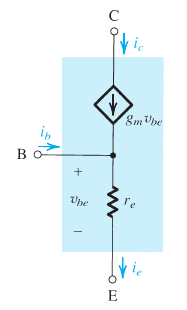
\includegraphics[scale=0.75]{./BJT-T_Small_Signal-vbe.png}
    \caption{T-Model Small-Signal Model, using $\ACVoltage{\pi}$\\\parencite[p.~409]{sedraTextbook7}}
    \label{fig:BJT-T_Model-vbe}
  \end{subfigure}
  \begin{subfigure}{0.45\linewidth}
    \centering
    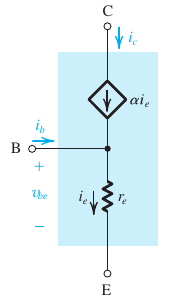
\includegraphics[scale=0.75]{./BJT-T_Small_Signal-alpha_ie.png}
    \caption{T-Model Small-Signal Model, using $\ACCurrent{\Base}$\\\parencite[p.~409]{sedraTextbook7}}
    \label{fig:BJT-T_Model-ib}
  \end{subfigure}
  \caption{Small-Signal Models of a \nameref*{def:BJT}}
  \label{fig:BJT-Small_Signal_Models}
\end{figure}

\begin{figure}[h!tbp]
  \centering
  \begin{subfigure}{0.45\linewidth}
    \centering
    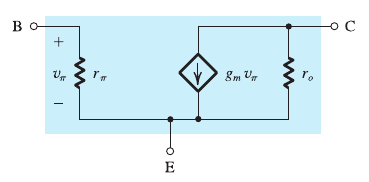
\includegraphics[scale=0.75]{./BJT-Hybrid_Pi-vbe-ro.png}
    \caption{Hybrid-$\pi$ Model Small-Signal Model, using $\ACVoltage{\pi}$ \parencite[p.~408]{sedraTextbook7}}
    \label{fig:BJT-Hybrid_Pi_Model-vbe-ro}
  \end{subfigure}
  \begin{subfigure}{0.45\linewidth}
    \centering
    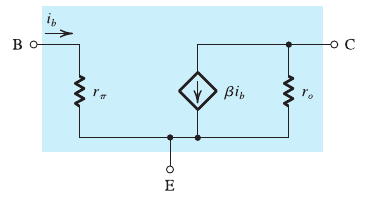
\includegraphics[scale=0.75]{./BJT-Hybrid_Pi-beta_ib-ro.png}
    \caption{Hybrid-$\pi$ Model Small-Signal Model, using $\ACCurrent{\Base}$ \parencite[p.~408]{sedraTextbook7}}
    \label{fig:BJT-Hybrid_Pi_Model-ib-ro}
  \end{subfigure}
  \\
  \begin{subfigure}{0.45\linewidth}
    \centering
    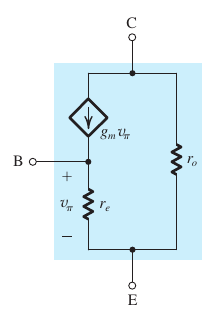
\includegraphics[scale=0.75]{./BJT-T_Small_Signal-vbe-ro.png}
    \caption{T-Model Small-Signal Model, using $\ACVoltage{\pi}$ \parencite[p.~410]{sedraTextbook7}}
    \label{fig:BJT-T_Model-vpi-ro}
  \end{subfigure}
  \begin{subfigure}{0.45\linewidth}
    \centering
    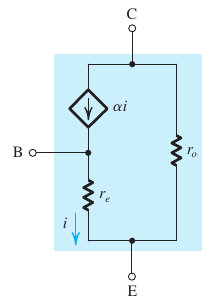
\includegraphics[scale=0.75]{./BJT-T_Small_Signal-alpha_ie-ro.png}
    \caption{T-Model Small-Signal Model, using $\ACCurrent{\Base}$ \parencite[p.~410]{sedraTextbook7}}
    \label{fig:BJT-T_Model-ib-ro}
  \end{subfigure}
  \caption{Small-Signal Models of a \nameref*{def:BJT}, including channel modulation resistance}
  \label{fig:BJT-Small_Signal_Models-ro}
\end{figure}

\begin{remark*}[Why T-Model?]
  The T-models are preferred when there is a resistor attached to the emitter of the \nameref{def:BJT}.
\end{remark*}

\subsubsection{Configurations}\label{subsubsec:BJT_Configurations}
The three possible configurations for a \nameref{def:BJT} are shown in \Crefrange{fig:BJT-Common_Emitter}{fig:BJT-Common_Collector}.

\begin{figure}[h!tbp]
  \centering
  \begin{subfigure}{0.30\linewidth}
    \centering
    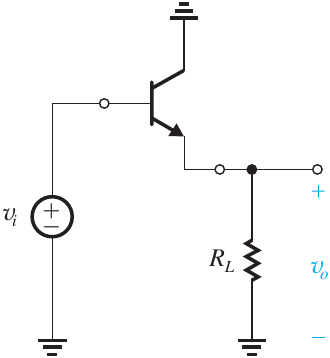
\includegraphics[scale=0.50]{./BJT-Common_Emitter.png}
    \caption{Common Emitter Configuration\\\parencite[p.~424]{sedraTextbook7}}
    \label{fig:BJT-Common_Emitter}
  \end{subfigure}
  \begin{subfigure}{0.30\linewidth}
    \centering
    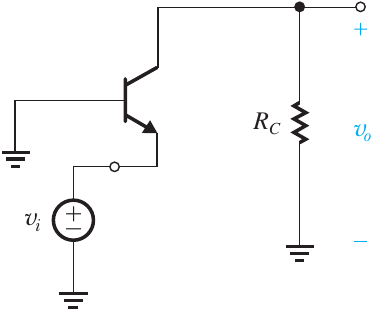
\includegraphics[scale=0.50]{./BJT-Common_Base.png}
    \caption{Common Base Configuration\\\parencite[p.~424]{sedraTextbook7}}
    \label{fig:BJT-Common_Base}
  \end{subfigure}
  \begin{subfigure}{0.30\linewidth}
    \centering
    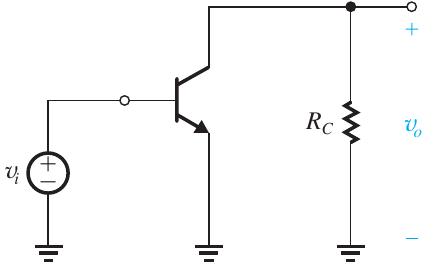
\includegraphics[scale=0.50]{./BJT-Common_Collector.png}
    \caption{Common Collector Configuration\\\parencite[p.~424]{sedraTextbook7}}
    \label{fig:BJT-Common_Collector}
  \end{subfigure}
  \caption{\nameref*{def:BJT} Configurations}
  \label{fig:BJT_Configurations}
\end{figure}

\subsection{Amplification}\label{subsec:Amplification}
The \emph{amplification} of a circuit is the ratio of the measured output against its input.
\Cref{eq:Amplification} illustrates this.

\begin{equation}\label{eq:Amplification}
  \Amp{} = \frac{\ACVoltage{\Out}}{\ACVoltage{\In}}
\end{equation}

\subsection{Gain}\label{subsec:Gain}
The \emph{gain} of a circuit is determined by the ratio of the output signal when a load is attached to the input signal.
This is distinctly different than \nameref{subsec:Amplification} because a load resistance has been added, which alters the output signal.

\Cref{eq:Gain} gives a general equation for the gain of a circuit.
\textbf{Remember that $\ACVoltage{\Out}$ MUST include the load resistance!}
\begin{equation}\label{eq:Gain}
  \Gain{} = \frac{\ACVoltage{\Out}}{\ACVoltage{\In}}
\end{equation}

The gain of a circuit can be calculated by multiplying the amplification of various subcomponents in the circuit with each other.
Thus, \Cref{eq:Gain-Broken} can be put together.
\begin{equation}\label{eq:Gain-Broken}
  \Gain{} = \Amp{1 \to 2} \Amp{2 \to 3} \cdots \Amp{n-1 \to n}
\end{equation}

%%% Local Variables:
%%% mode: latex
%%% TeX-master: "../ECE_311-Engineering_Electronics-Reference_Sheet"
%%% End:
